\documentclass{article}
\usepackage{amssymb, amsmath}
\usepackage{graphicx}
\usepackage{epstopdf}
\usepackage[utf8]{inputenc}
\usepackage{mdwlist}
\usepackage[left=1cm, right=2cm, top=1.5cm, bottom=1.2cm]{geometry}
\epstopdfsetup{outdir=./}
\begin{document}

  \begin{enumerate*}
    \item [1.]
    \begin{enumerate*}  
      \item [(a)] \text{}\\
      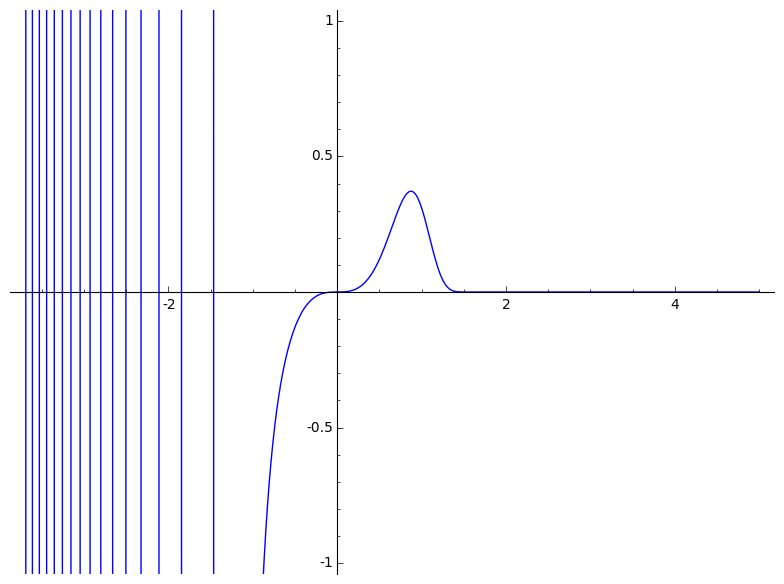
\includegraphics[width=0.7\textwidth]{$PWD/Q1_1.png}

	  \item [(b)] \text{}\\ 
      The (a) figure show that the value of y will be changed in large range(from positive infinity to negative infinity) between x-value -1 to -5. Therefore, we cannot calculate accurate answer for this formular and we cannot get a numeracal answer.
      
      \item [(c)] \text{}\\ 

    \end{enumerate*}
    
    \item [2.]
    \begin{enumerate*}
      \item [(a)]
      $\because$ p is prime, and p is coprime between all integers from 1 to p except number 1 \\
      $\therefore \ phi(p)\ is\ p-1$ 
      
      \item [(b)]
      Obervation: \\
      $\phi(11) \times \phi(13) = \phi(11 \times 13)$ \\
      In my opinion, all distinct prime numbers p and q can be done by this observation because p and q are different numbers and they are coprime.
      
      \item [(c)]
        \ 
        \begin{enumerate*}
          \item [(i)]
          Suppose we have distinct prime number p and q.
          
          \item [(ii)]
          $\because$ p is prime number, and q is also prime number \\
          $\therefore\ \phi(p) = p-1,\ \phi(q) = q-1,\ \phi(p)\phi(q)=(p-1)(q-1)$

            
           
        \end{enumerate*}
    \end{enumerate*}
  \end{enumerate*}
\end{document}

